\documentclass{standalone}

\usepackage{graphicx}

\usepackage{tikz}

\usetikzlibrary{positioning}
\usetikzlibrary{arrows.meta}
\usetikzlibrary{calc}

\begin{document}

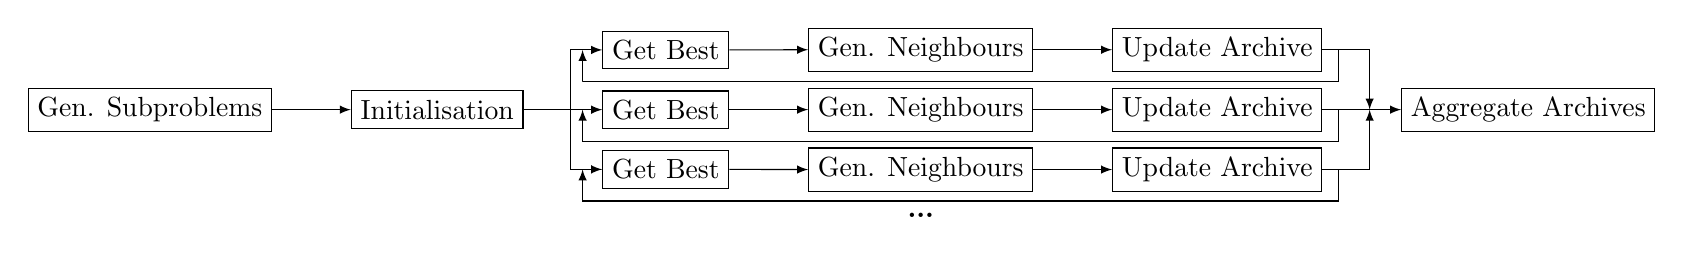
\begin{tikzpicture}[
    block/.style={rectangle, draw=black, fill=white},
]
    \node[block] (B1) [] {Gen. Subproblems};
    \node[block] (B2) [right=of B1] {Initialisation};

    \node[block] (BA3) [right=of B2] {Get Best};
    \node[block] (BA4) [right=of BA3] {Gen. Neighbours};
    \node[block] (BA5) [right=of BA4] {Update Archive};

    \node[block] (BB3) [above=0.27cm of BA3] {Get Best};
    \node[block] (BB4) [above=0.2cm of BA4] {Gen. Neighbours};
    \node[block] (BB5) [above=0.2cm of BA5] {Update Archive};

    \node[block] (BC3) [below=0.27cm of BA3] {Get Best};
    \node[block] (BC4) [below=0.2cm of BA4] {Gen. Neighbours};
    \node[block] (BC5) [below=0.2cm of BA5] {Update Archive};

    \node[] () [below=0.15cm of BC4] {\textbf{...}};

    \node[block] (B6) [right=of BA5] {Aggregate Archives};

    \draw[-latex] (B1.east) -- (B2.west);

    \draw[] (B2.east) -- ($(B2.east)+(0.6,0)$);
    \draw[-latex] ($(B2.east)+(0.6,0)$) -| ($(BA3.west)+(-0.4,0)$) -- (BA3.west);
    \draw[-latex] ($(B2.east)+(0.6,0)$) -| ($(BB3.west)+(-0.4,0)$) -- (BB3.west);
    \draw[-latex] ($(B2.east)+(0.6,0)$) -| ($(BC3.west)+(-0.4,0)$) -- (BC3.west);

    \draw[-latex] (BA3.east) -- (BA4.west);
    \draw[-latex] (BA4.east) -- (BA5.west);

    \draw[-latex] (BB3.east) -- (BB4.west);
    \draw[-latex] (BB4.east) -- (BB5.west);

    \draw[-latex] (BC3.east) -- (BC4.west);
    \draw[-latex] (BC4.east) -- (BC5.west);

    \draw[] (BA5.east) -| ($(B6.west)+(-0.4,0)$);
    \draw[-latex] (BB5.east) -| ($(B6.west)+(-0.4,0)$);
    \draw[-latex] (BC5.east) -| ($(B6.west)+(-0.4,0)$);
    \draw[-latex] ($(B6.west)+(-0.4,0)$) -- (B6.west);

    \draw[-latex] (BA5.east) -| ($(BA5.east)+(0.2,-0.4)$) -| ($(BA3.west)+(-0.25,-0.4)$) -- ($(BA3.west)+(-0.25,0)$);
    \draw[-latex] (BB5.east) -| ($(BB5.east)+(0.2,-0.4)$) -| ($(BB3.west)+(-0.25,-0.4)$) -- ($(BB3.west)+(-0.25,0)$);
    \draw[-latex] (BC5.east) -| ($(BC5.east)+(0.2,-0.4)$) -| ($(BC3.west)+(-0.25,-0.4)$) -- ($(BC3.west)+(-0.25,0)$);
\end{tikzpicture}

\end{document}